\documentclass[11pt]{article}
%\usepackage{fontspec}
\usepackage{ amssymb }
\usepackage{longtable}
\usepackage{amsmath}
\usepackage{graphicx}
%\usepackage[utf8]{inputenc}
\author{Raghav Kuppan, Lee Richert, and Yuanda Zhu}
\title{Project Final Report}
\begin{document}

\begin{center}
\textbf{\Large Learning the structure of a Markov Random Field}
\end{center}

\begin{center}
Lee Richert (ECE), Raghav Kuppan (ECE), Yuanda Zhu (ECE)
\end{center}



\section{Abstract}
Learning the structure of a Markov Random Field from independent and identically distributed samples is an important problem.
Unfortunately, calculation of the partition function is intractable for most graphs.
Trace Lasso regularization of a pseudo-likelihood has been proposed as a means of learning the structure of probabilistic graphical models from samples. 
The Trace Lasso exhibits less volatility in response to correlation between random variables than Lasso while also promoting sparsity. 
We use Trace Lasso for the purpose of learning the structure of a Markov Random field, using a maximum pseudo-likelihood approach.


\section{Introduction}

Ising models are most well known for their original application of modeling ferromagnetism in statistical mechanics, but their utility spans far beyond that narrow application.
Interactive binary variables occur frequently in biological data, especially dealing with genetics \cite{wang2009learning}\cite{rhemtulla2016network}\cite{mcnally2015mental}
In the field of psychopathology, researchers use Ising models to identify core symptoms and guide further investigation into the origin, persistance, and collapse of psychological disorders\cite{fried2016good}.
Surpisingly, despite the existance of better-suited algorithms to deal with binary data, many researchers still use graphical lasso, the optimal algorithm for learning Gaussian Markov Random Fields, but a poor fit for learning Ising models.

Learning the maximum likelihood structure of binary, pairwise systems is an NP-hard problem, even with complete data.
To make things tractable, we use a pseudolikelihood approximation and maximize pseudolikelihood factors.  

\subsection{Defining the Ising Model}
An Ising Model is as special case of a pairwise Markov Random Field where each vertex in the graph takes on values in \{-1,1\}.
The node potentials and edge potentials for an Ising model have very simple expressions thereby giving us a distribution of the form
\[ \mathbb{P}_{\theta^*} (x)  =  \frac{1}{\mathbb{Z(\theta}^*)} exp { \sum\limits_{ (s,t) \in E} \theta^*_{st} x_s x_t  }   \]

The Ising Model was proposed as a mathematical model for ferromagnetism in statistical mechanics but is also used in other applications such as Computer Vision and Neuroscience.

	

\section{Prior Work on Model Selection}

Learning the structure of Ising models is a challenging problem. 
For a general graph with $p$ nodes of degree at most $ d $, an exhaustive search across all possible edges takes around $ p^d $ computations. 
This is the time required to exhaustively search over all possible neighborhooods of a node and for each node test whether conditional independence assumptions hold. 
As $ d $ grows, the computational cost becomes untenable, so algorithms with lower computational complexity are desired.
In general, efficient algorithms for structural learning either restrict the graph structure or the nature of the interactions between the nodes. 
One possible assumption of the second kind is the Correlation Decay Property. 
A graphical model is said to have the correlation decay property if any two variables are asymptotically independent as the graph distance between them increases. 
This property holds for Ising models in certain real-world problems such as the ferromagnetic model in a high temperature regime. 
Alternative methods that do not explicitly require the Correlation Decay Property are usually based on Convex Optimization. \\

Ravikumar et. al ~\cite{ravikumar2010high} study the problem of signed edge recovery on Ising models and propose an $l_1$-regularized logistic regression approach to recover the signed edges in the graph.
They establish sufficient conditions on the sample size $n$, dimension $p$, and maximum neighborhood size $d$, to get a consistent estimator.
With this assumption, the structure of any bounded degree graph can be recovered with high probability once $n/log(p)$ is sufficiently large. 
This way, the signed neighborhood of every node can be estimated by optimizing a log pseudo-likelihood function with an $\ell_1$ penalty.
This way the entire set of signed edges of the graph can be recovered whereby the structure of the Ising model has been found.
This technique is demonstrated on four-nearest neighbor lattices, eight-nearest neighbor lattices and a star graph as well as on a class of graphs with unbounded maximum neighborhood size, with the results being consistent with the theoretical conjectures


\subsection{Pseudolikelihood Functions}

A Pseudolikelihood is an approximation to the likelihood function which provides a computationally simpler model for inference in a graphical model and is also exact provided certain assumptions are made about the model. 
The Ising model joint probability expression cannot be exactly computed since the partition function makes computations intractable.
Our method involves computing a regularized-pseudolikelihood factor for each node $X_r$ conditioned on the other nodes.
The pseudolikelihood approach involves computing the conditonal distribution of a node conditioned on all the other nodes, and then performing the optimization over the parameter set.
As we are dealing with the Ising model, the conditional distribution has a very clean expression given as 
$$ \mathbb{P_{\theta^*}}( x_r | x_{\backslash r})  $$ 
Provided we have samples from the graphical model, this expression is easily computed.\\
Therefore, given a set of independent and identically distributed samples,  each regularized pseudolikelihood factor is of the form of a convex program 
$$ \min_{\theta_{\backslash r} \in \mathbb{R}^{p-1}} \{ l(\theta; \mathbb{X}^n_1) + \lambda \|{ \theta_{\backslash r} }\| \} $$

where $\mathbb{X}^n_1)$ is the set of i.i.d samples from the graph and $\lambda$ is the regularization hyperparameter. 

Different regularization techniques can be used according to the correlation structure of our data and the application where the Ising model is being used.

\subsection{Regularization}

Regularization is a method to avoid the overfitting problem in Machine Learning. 
In our case, it takes the form of a feature selection problem and is used to get a sparse approximation for our optimization. 
This makes our model cheaper and more interpretable. 
Among sparsity inducing norms, the $\ell_1$ norm is the simplest and most widely used, leading to the Lasso when used in a least-squares framework.
While the Lasso does well in high-dimensional settings, it is known to have stability problems in situations where the data exhibit strong correlation structures. 
Several solutions have been proposed which include the Elastic net, group Lasso and Sampling techniques. 
However these norms cannot just be plugged into the objective function as extra information is usually required, or in some cases, the problem is further complicated due to the addition of parameters to be estimated. 
The Trace norm takes into account the correlation structure of the data but does not require manual human intervention. 
It can be thought of as a way of turning the rank of a matrix into a norm. The Trace norm is adaptive and requires that only a single regularization parameter be chosen. 	


\subsubsection{Lasso}

Penalizing linear models by the number of variables used in the model is a method of variable selection in sparse high-diensional settings. 
As this criterion is not convex, a convex relaxation for this norm is the $\ell_1$ norm. 
But a solution to the likelihood function penalized with this penalty is not equivariant to the rescaling of the predictors, so it is common to normalize the predictors. 
When normalizing the predictors and penalizing with the Lasso, we are implicitly using a regularization term that depends on the data matrix. 
We can write the normalized $\ell_1$ norm as 
$$ \|\mathbf{\theta}\|_1 = \sum \limits_{i=1}^p \|{\mathbf{X}^i}\|_2 |\theta_i| $$ 

But the Lasso is known to perform poorly under three conditions:

\begin{enumerate} 

\item

Let $p$ represent the number of features and $n$ represent the number of observations. For $p>n$, Lasso selects at most $n$ variables before it saturates; besides, Lasso is not well defined unless the bound on $\ell_1$-norm of the coefficients is smaller than a certain value.
\item

For a group of variables whose pairwise correlations are very high, Lasso tends to select only one variable and does not care which one is selected.

\item

 For $n>p$ case, when predictors have high correlations, the prediction performance of Lasso is dominated by ridge regression.\\ \\
 \end{enumerate}


\subsubsection{Group Lasso}

Group Lasso divides the predictors into groups and penalize the sum of the `$\ell_2$ norm of these groups.
The Group Lasso is especially useful in case our model contains categorical variables. 
In case of categorical variables, the Lasso might leave out some levels in the category, as discussed in the previous section. 
The Group Lasso provides a method to incorporate prior information about the categories available.
Given a partition set ($S_i$), the group Lasso can be calculated as
$$ \|\mathbf{\theta}\|_{GL} = \sum \limits_{i=1}^k \|\theta_i\|_2 $$

The effect of this penalty function is to introduce sparsity at the group level: variables in a group are
selected all together.
The drawback here is that the Correlation structure of the data or information about the category partition must be known a priori. 
\subsubsection{Elastic Net}

In order to address the third problem of Lasso, elastic net ~\cite{Zou2005Reg} was proposed in 2005 by adding the squared $\ell_2$ norm, a strongly convex penalty term to the $\ell_1$ norm in Lasso. 
Elastic net performs similarly to Lasso in scenario 1) and 2), but by encouraging grouping effect, has higher accuracy than Lasso in scenario 3). 
To be more specific, in scenario 3), some features are highly correlated with each other and are associated with response; thus elastic net aims to perform less shrinkage on those subsets of features. 
In addition, similar to Lasso, elastic net does both continuous shrinkage and automatic variable selection. Ridge regression has only continuous shrinkage but no automatic variable selection.\\


\subsubsection{Trace Lasso}

The Trace norm is a measure of the dimension of the subspace spanned by the selected predictors.
The trace norm of a matrix is the sum of its singular values. 
The Trace lasso can be defined as $\| \mathbf{X} Diag(\mathbf{\theta})\|_*$
It has some interesting properties;
\begin{enumerate}
\item  If all the predictors are orthogonal, then, it is equal to the $\ell_1$ norm.
\item  If all the predictors are equal, then, it is equal to the $\ell_2$ norm
\end{enumerate}

Thus when two predictors are strongly correlated, our norm will behave like
Tikhonov regularization, while for almost uncorrelated predictors, it will behave like the Lasso.

Instead of blindly adding convexity in all directions, the trace lasso adds strong convexity only in the direction of highly correlated predictors. 
Thus, it always has a unique minimum and is much more stable than the lasso. 
\section{Approach}

Our approach is to adopt the maximum psuedo-likelihood approach as in~\cite{ravikumar2010high} but with the trace norm as our regularization parameter. 
The signed neighborhood of one node will be estimated by evaluating the conditional distribution of the node conditioned on all the other nodes and then maximizing this with a trace norm penalty.
Computing the Pseudo-likelihood using the generated samples is not very hard for the Ising model. 
However there are some difficulties in evaluating the trace norm. 
The usual method of optimization is by subgradient descent where the subgradient is the generalization of the derivative to functions which are not differentiable. 
Computing the subgradient of the trace norm is reported to be inefficient and the rate of convergence very slow, so a variational formulation for the trace norm~\cite{grave2011trace} is be used. 
The ensuing cost function can be optimized using a Conjugated Gradients method.\\ \\
The Trace Norm of a matrix $M$ can be expressed as 
$$ \|M\|_* = \frac{1}{2} \underset{S \succeq 0}{inf} \quad  tr(M^T S^{-1} M) + tr(S)	 $$
and the infimum is attained for $S = M^T M$.\\ \\
Therefore, our optimization problem can be reformulated as
$$ \min_{\theta_{\backslash r} \in \mathbb{R}^{p-1}}  l(\theta; \mathbb{X}^n_1) + \frac{\lambda}{2} \theta^T Diag(diag(X^T S^{-1} X ))\theta + \frac{\lambda}{2} tr(S) $$ 
where $Diag(u)$ is the diagonal matrix whose diagonal elements are the vector $u$ and $diag(M)$ is the diagonal of the matrix $M$.
This problem is jointly convex in $(\theta, S)$ and con be solved by alternating the minimization over $\theta$ and $S$.
The matrix $S$ can be computed with a closed form expression for the given problem which leaves us with a convex optimization program for the parameter $\theta$.
This can be solved using a conjugated gradients method. The optimization is still not cheap as compared to the $\ell_1$ norm and takes quite some time to run. 

%\subsection{Parameter Selection}
\subsection{Applying Methods to Categorical Data}
Categorical data with more than two categories is not binary.
However, a variable with $m$ disjoint categories can be treated as $m - 1$ binary random variables (the last category is the negative of all other categories).
Pairwise connections can be learned on the expanded model as if it were an Ising model.
Interaction between within-variable nodes are not pairwise, and should not be treated as such, but it is not unreasonable to model between variable interactions as pairwise interactions between the binary nodes.
This allows us to attack categorical problems with the algorithms described in earlier sections.
For more details, see \cite{ravikumar2010high}.  


\subsection{Learning Graphical Models for Classification}
% This is the appropriate subsection for comparison to logistic regression
A pseudolikelihood factor is the expression used in logistic regression. We wondered if by leveraging the arguments maximizing other pseudolikelihood factors could be used to improve upon pseudolikelihood regression (through symmetry enforcement). We attempt this in the experiments section using the Wainwright minimum \cite{hoffling2009estimation}. 

Noteably, this type of approach would not require finding the arguments maximizing all of the pseudolikelihood factors, because sparsity-encouraging regularization likely would remove some of the edges incident to the node of interest. Only factors containing the remaining edges would need be considered. That is, we only need to consider the pseudolikelihood factors corresponding to nodes selected by the pseudolikehood function of the node of interest. This allows for some computational savings.

\section{Datasets}

For Ising model, appropriate real world datasets are not easy to find, since possible choices on one subject are not usually limited to two. Thus, besides the congressional voting record data set, which after eliminating missing votes, we have nicely binary values for the voting pattern of each bill, all other data sets would have three or more possible values for each attribute. We then examined through the categorical data through UCI Machine Learning Repository ~\cite{Dua:2017}. We found the mushroom data set specifically interesting, due to its large number of samples, as well as its 22 attributes that together contribute to whether one specifically given mushroom is poisonous or edible.

\subsection{Congressional Votes}

During the Congressional Quarterly Almanac, 98th Congress, 2nd session, 1984, 435 U.S. House of Representatives Congressmen voted on 16 bills. For each bill, every single congressman or congresswoman could vote for it, against it, or abstained. Abstained votes are considered as missing data. For the past 30 years, over 20 publications have cited this data set. Some papers focused on feature selection ~\cite{Chun1999ANNigma} ~\cite{Huan1998Inc}, others related to decision tree ~\cite{Erin1995Fea} and budgeted learning ~\cite{Dan2012Bud}. For our project, instead of researching the relationship between each congressman, we explored the interaction between bills. To be more specific, we would query the possibility of how a congressman (democrat or republican) would vote on a single bill given the pattern of other 15 bills.

\subsection{Mushroom Data}

Different from congressional votes data set, this mushroom data set "includes descriptions of hypothetical samples corresponding to 23 species of gilled mushrooms in the Agaricus and Lepiota Family (pp. 500-525)". 22 attributes are included; each attribute has possible values ranging from 2 to 12. The goal for this data set is much clearer than the congressional votes data set: all we need to know is how these attributes together would decide whether the mushroom is edible. Notice that there is no simple rule to determine the edibility of a mushroom. Comparing with the congressional votes data set, another advantage of this data set is that it has more than 8000 samples; what's more, all missing data are on the 11th attribute, so that we can either completely remove the 11th attribute from our modeling or treat the missing data as an extra value. For this data set, 46 publications are dated. Most of them are related to machine learning, data mining and feature selection.

\section{Logistics}

Cleaning of the data and other basic data processing was done on the samples from the dataset using Python. This step also included the removal of samples with missing data from the dataset. 
The Pseudo-likelihood optimization with regularization was done in Python using the NumPy and SciPy libraries. 
More specifically, the \textit{minimize} procedure from the \textit{optimize} library was used for the Conjugated Gradients method. 
The lasso, trace lasso and the elastic net were the regularization schemes implemented in the program.

We coded the Gibbs block sampling code in MATLAB, and coded a second version of the trace Lasso maximum pseudolikelihood code in MATLAB for compatibility with the Gibbs sampling code. The PGM_factor class and all other code we submit was written by us, and us alone.  The derivatives used in the MATLAB code are of our own derivation, and the optimization routines are our own code as well. The novelty of using only some of the pseudolikelihood factors for classification is of our own design.

\section{Experiments}
\subsection{Synthetic Data}
On a $8\times8$ degree-$4$ planar lattice, we generate the weights and individual node biases independently from a unit-variance, zero-mean Gaussian distribution.
We use Gibbs sampling to generate samples.
Then, we use those samples to attempt to reconstruct the graph. We consider an edge to be "recovered" if its weight is of the same sign as the generating graph.

Unfortunately, the edge recovery under trace LASSO was essentially random. There is a tradeoff between stability and encouraging sparsity. While Trace Lasso does enourage sparsity to an extent, it appears this was insuffient for edge recovery.
  
\subsection{Congressional Voting Data}

In Datasets Section, we mentioned about the three possible outcomes for each bill from the congressmen. In order to feed the data into our Ising model, we removed all samples of congressmen whose voting records included missing data. In this way we limited only two possible outcomes for each bill. As a result,  232 samples of congressmen remained. 

We further divided these 232 congressmen into two sections, based on their party. 80 percent of data in each section are our training data, to be fed into one of the three core algorithm: Lasso, Trace Lasso and Elastic Net. Ising model was built with the parameters optimized from the core algorithm. The rest 20 percent of the data are our testing data; they were queried with the Ising model to calculate the likelihood. 

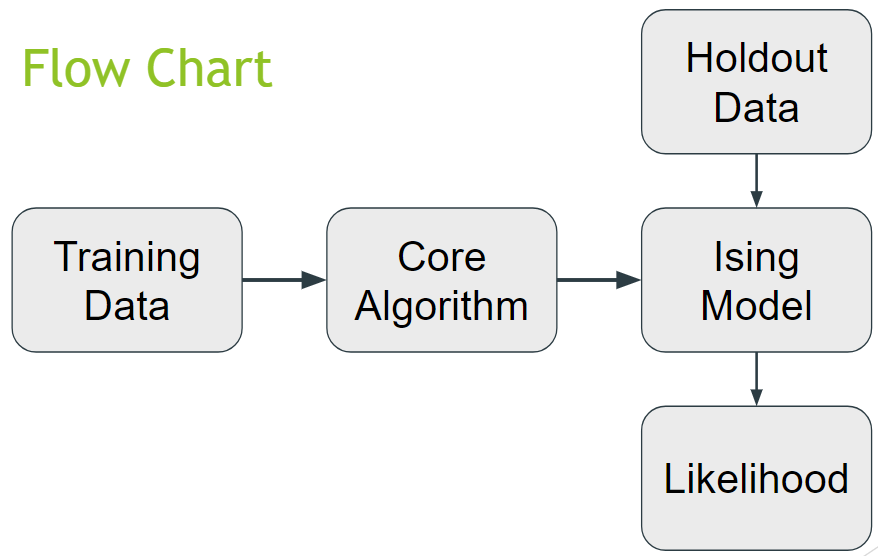
\includegraphics[scale=0.5]{Control_Flow}

Since we would like to know how the bills interact with each other, our goal was to predict how the congressman would vote on a target bill given the voting pattern of all other 15 bills. Thus, for our Ising model, each bill is a node; a total of 16 nodes are in the graphical model. Also note that two separate Ising models were generated, one for democrats and the other for republicans.

We predict the voting pattern for target bill against all samples in our hold out sets. Accuracy is calculated based on correct prediction out of total prediction. Each single bill has each own accuracy value. We take the average of accuracy of all 16 bill to evaluate the overall performance of one core algorithm. 

\
\begin{table}[ht]
\centering
\begin{tabular}{c c c c}
\hline
Accuracy & Trace Lasso & Lasso & Elastic Net \\
\hline
Democrat & 0.57 & 0.48 & 0.47 \\
Republican & 0.62 & 0.44 & 0.49 \\
\hline 
\end{tabular}
\caption{Accuracy for Three Core Algorithms.}
\label{table:nonlin} 
\end{table}

As we can see from the table, Trace Lasso has roughly 10 percentage higher accuracy than the other two algorithms. Still, the accuracy of Lasso and Elastic Net is quite low, even lower than tossing a fair coin. We noticed that Ising model might not be a good graphical model to interpret the interaction between bills.


\
\begin{table}[ht]
\centering
\begin{tabular}{c c c c}
\hline
Algorithm & Trace Lasso & Lasso & Elastic Net \\
\hline
Computational Time & 636 sec & 55 sec & 67 sec \\
\hline 
\end{tabular}
\caption{Computational Cost for Three Core Algorithms.}
\label{table:nonlin} 
\end{table}

On the other hand, Trace Lasso is at much higher computational cost. We ran three trials for each algorithm, and took the average time. It is observed that Trace Lasso roughly requires 10 times as much as computational time.

\subsection{Mushroom Data}
\section{Conclusions}
While in some cases Trace Lasso may outperform competing methods, its overall performance is underwhelming. The cost of computing the singular value decomposition for an $N\times N$ matrix (where $N$ is the number of samples) will in most instances outweigh any potential gains from using this particular penalty term.
\section{Acknowlegements}
We would like to acknowlege Professor Fekri for including this idea in the list of suggested projects.

\bibliography{citation}{}
\bibliographystyle{plain}

\end{document}

